\documentclass{mcmthesis}
\mcmsetup{CTeX = true,
        tcn = 83451, problem = A,
        sheet = true, titleinsheet = true, keywordsinsheet = true,
        titlepage = false, abstract = false}
\usepackage{palatino}
\usepackage{graphicx}
\usepackage{url}
\title{ The solve of MCM 2018 problem A }
\author{\small Team \# 83451}
\date{\today}
\begin{document}

\begin{abstract}

waiting to add!

\begin{keywords}
  Try; Table; Picture; Reference
\end{keywords}
\end{abstract}
\maketitle

\tableofcontents
\newpage

\section{Introduction}

\subsection{Motivation}

On a sunny summer day, everyone wants to enjoy the pleasure of fishing on a yacht at sea. However, as we enter the deep ocean, chances are that our on-board HF(3-30MHz) receiver was unable to receive timely broadcast warnings of the coming bad weather from the Maritime Bureau, then our wonderful summer afternoon would be destroyed by the ensuing storm. Based on the current HF broadcast model, which consists a blind area, such stories will be staged on the sea for many years.

\subsection{Problem Restatement}


\section{General Assumptions}

    To simplify the real life situation, we will accept the following assumptions while we construct our models.

    \begin{itemize}

      \item a. We assume that the transmitting antenna radiates a particular frequency of spherical waves.

      \item b. According to the far propagating distance, the Earth-surface cannot be considered as a plane, which we always do to handle some daily problems. However, we can approximate the Earth  to a sphere with a radius of 640,000 km. In addition, \textbf{the ionosphere and the ocean are in concentric spheres}.

      \item c. Due to the facts that the light wave is one kind of \textbf{electromagnetic waves (EM waves)}, we assume that the ionosphere and the ocean's reflection of EM waves can be analyzed using the same method as \textbf{geometrical optics}.

      \item d. Suppose the temperature and pressure in the entire propagation space path are almost constant, which means we will ignore the loss of EM waves caused by flowing air or non-constant physical characters (especially the temperature and pressure).

      \item e. We will not justify the electromagnetic noise from the radio receiver. We will assume that the noise mainly comes from the atmosphere.

    \end{itemize}

\section{Constants and Notations}

    In order to calculate and describe our mathematical model more simply and clearly, we will use the following mathematical notation, where the values we assume or determine as constants will give its values and units here in Table \ref{tab:Constants}. Some of the units such as \emph{$dB$ and $dBm$} is not easy to see in other field. The details of these less commonly used units will be discussed later.

    \begin{table}[h]
      \centering
        \begin{tabular}{|c|c|c|}

          \hline Constants & Definition & Value (with units) \\
          \hline $P_{initial}$ & How much energy does the initial HF signal has & $100(W)$ \\
          \hline

        \end{tabular}
        \caption{Constants}
        \label{tab:Constants}
    \end{table}


    \begin{table}[h]
      \centering
        \begin{tabular}{|c|c|l|}

          \hline Notations & Definition & Unit \\
          \hline $E_{r}$ & How much energy may trasmit to the receiver & $dBm$ \\
          \hline $E_{g}$ & How much energy will be generated & $dBm$ \\
          \hline $G_{r}$ & The antennas gain of receiver & $dBi$ \\
          \hline $G_{g}$ & The antennas gain of generator & $dBi$ \\
          \hline $L_{totle}$ & The totle energy loss during the propagation & $dB$ \\
          \hline $L_{fspl}$ & The free space path loss & $dB$ \\
          \hline $L_{a}$ & The loss during passing the ionosphere layer & $dB$ \\
          \hline $L_{gd}$ & The loss during the reflection on the grond & $dB$ \\
          \hline $L_{addition}$ & Additional loss of the signal energy & $dB$ \\
          \hline

        \end{tabular}
        \caption{Notations}
    		\label{tab:Notations}
    \end{table}



\section{High Frequency Electromagnetic Waves}
  \subsection{High Frequency Electromagnetic Waves (HF-EM waves).}

    The electromagnetic wave, in physics, refers to the wave of the electronic field, propagating through space-time, carrying electromagnetic radiant energy. Classically, we can just study one component of the electromagnetic wave to represent the physical state of the entire wave. And the EM waves can be described as:

      \begin{equation}\label{eq:EMW}
        E = A * \cos(\omega t + \phi_{0})
      \end{equation}
      Where: \\
      $E$ is represent the electric field strength; \\
      $\omega$ is the angular frequency;\\
      $t$ represents how much time has passed since the wave had been generated;\\
      $\phi_{0}$ is the initial phase of the wave.\\

      And for studying the physical properties and changes of electromagnetic fields, we introduce the classical Maxwell equations:


      \begin{equation}\label{eq:Maxwell_new}
      \left\{
      \begin{aligned} % \begin{eqnarray}好像也可以。
          \nabla \times \textbf{H}  &= \textbf{J} + \frac{\partial\textbf{D}}{\partial t}       \\
          \nabla \times \textbf{E}  &= -\frac{\partial\textbf{B}}{\partial t}       \\
          \nabla   \cdot  \textbf{B}  &= 0       \\
          \nabla   \cdot  \textbf{D}  &= \rho
      \end{aligned}
      \right.
      \end{equation}
      The mathematical notations in this Equationa are the same as the habitual use of physical formulas


      As we known, \textbf{high frequency (HF)} is the designation for the range of radio frequency EM waves between 3 and 30 megahertz (MHz). The most interesting and important property of this frequency band, is that it can be reflected in the ionosphere layer in the atmosphere — a method which named \emph{sky wave} or \emph{skip}. It is because that the ionized atoms in the atmosphere can interact with HF-EM waves to change its radiating path.\cite{HF_EM}

      If the sky wave which reflected to the Earth can be reflected again by the ground, a \emph{multi-hop propagation} model would be formed between the ionosphere and the Earth-surface(Figure ~\ref{fig:Multi_hop}). Depending on multi-hop propagation, the scope of the HF communications has been greatly enhenced.

      \begin{figure}[ht]
      \centering
      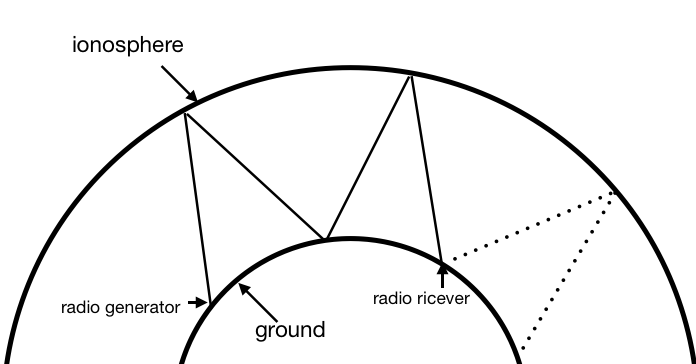
\includegraphics[scale=0.5]{Multi_hop}
      \caption{The Multi-hop propagation}
      \label{fig:Multi_hop}
      \end{figure}


  \subsection{HF-EM waves Propagation Model}

    Based on the modern physics common knowledge, HF-EM waves use the energy of the electromagnetic field to transmit information. So we can determine the signal strength by simply considering its enery. Especially in the radio-related applications, we usually use the unit known as decibel(\emph{dB}) to represent the energy relation of radio wave generating, transmitting and receiving. The decibel is a logarithmic unit used to express the ratio of the physical property to another, and may be used to describe a change in the value we discussed. Normally, the method of using decibel to describe the power quantity is:

      \begin{equation}\label{eq:power_dB}
        N|_{dB} = 10 \lg(\frac{P_{i}|_{W}}{P_{0}|_{W}})
      \end{equation}
      Where: \\
      $N$ represents the decibel figure we need to describe the ratio of the \textbf{current power} $P_{i}$ to the \textbf{initial power} $P_{0}$.\\

    In this paper, we will adopt this unit to describe the loss of the power in both of the ionosphere and ocean surface. Since we are solving a radio-related issue, to simplify our calculation, we will also use a unit named as dBm (power relative to 1 milliWatt) to measure the power of our EM waves. By the Equation \ref{eq:power_dB}, we get:

      \begin{equation}\label{eq:dBm_milliWatt}
        E |_{dBm} = 10 \lg(\frac{P_{i}|_{W}}{1 |_{mW} })
      \end{equation}

    Because we always use $W(Watt)$ as the power units, so the following Equation is commonly used:

      \begin{equation}\label{eq:dBm_Watt}
        E |_{dBm} = 30 + 10 \lg(\frac{P_{i}|_{W}}{1 |_{W} })
      \end{equation}

    In order to simulate the performance of multi-hop HF-EM waves between the ionosphere and the ocean, we need to measure the physical condition of it. As a EM wave, the essential property is how much energy it has. So the rate of its energy loss is the key factor in accessing a signal propagation process. Using the derived Equation \ref{eq:dBm_Watt} and the unit(dB), the rate of the energy loss can be calculate like this:

      \begin{equation}\label{eq:transmitting}
        E_{r} = E_{g} + G_{g} - L_{totle} + G_{r}
      \end{equation}
      The characters we used has been discussed at Table \ref{tab:Notations}. Since the units \emph{$dBi$} and \emph{$dBm$} has the same meaning of \emph{$dB$}, we can put them together in one formular. The physics meaning of this Equation is easy to understand. As the \emph{$dB$} represents the logarithmic ratio of two number, the multiplications between the initial energy values and the ratios of gain and attenuation can be simply replaced by addition and subtraction.

    From the requirement, which directly give us the energy intensity($P_{initial} = 100 W $) of the initial EM wave, we can assume that the initial wave energy containing both of the generating energy and the gain. Then, using Equation \ref{eq:dBm_Watt}, we can get this result:

      \begin{equation}\label{eq:E_initial}
        E_{initial} = E_{g} + G_{g} = 50 (dBm)
      \end{equation}

    As for the loss of the enery $L_{totle}$, we assume the components of it are:

      \begin{equation}
        L_{totle} = L_{fspl} + L_{a} + L_{gd} + L_{addition}
      \end{equation}

     In this section, we will only study on the free-space path loss ($L_{fspl}$). And the details of other sections of the enery loss will be analyzed later.

  \subsection{Free-space Path Loss}

      The \textbf{free-space path loss(FSPL)}\cite{freespacepathloss} has been discussed for many years. FSPL can be used to calculate the signal strength loss when an EM wave travels over a line of sight path in free space. Based on the \emph{Assumption a} and exsting model of spherical waves in free space \emph{(between the ionosphere and the ground)}, we can draw the result of that:

        \begin{equation}\label{eq:FSPL_old}
          L_{fspl} = (\frac{4 \pi d f}{c})^{2}
        \end{equation}
        Where: \\
        $d$ is the distance of the receiver from the transmitter (metres)\\
        $f$ is the signal frequency (Hertz)\\
        $c$ is the speed of light in a vacuum (metres per second)\\

      If we use \emph{dB} as the unit, then we convert this formula to:

        \begin{equation}\label{eq:FSPL_applied}
          L_{fspl} = 20\log(d) + 20\log(f) + 32.44
        \end{equation}
        Where:\\
        $d$ is the distance of the receiver from the transmitter (km)\\
        $f$ is the signal frequency (MHz)\\

      \emph{Notice: the units we use in the Equation \ref{eq:FSPL_old} and Equation \ref{eq:FSPL_applied} are different. In the following Equations, except for special Notice, we will take the frequency unit as MHz}

      By applying this formular, the FSPL can be simply calculated if we have the value of free space distance and the frequency of our EM wave.

\section{The Ionosphere}

  \subsection{The Ionosphere Structure Model}
    The ionosphere is a shell of electrons and electrically charged atoms and molecules that surrounds the Earth, stretching from a height of about 50 km to more than 1,000 km. It exists primarily due to ultraviolet radiation from the Sun. Classically, ionosphere has four layers, which named D; E; F1 and F2 (from lower to higher), and each layer has its own unique physical property.\cite{davies1990ionospheric} Some basic information of the four layers is being displayed in Table \ref{tab: the ionosphere layers}.

        \begin{table}
          \centering
            \begin{tabular}{|l|l|l|}
            \hline
            Layers                  &Day & Night      \\ \hline
            F2 (lower than 500 km)  & The main reflection layer for HF waves & combine with F1          \\ \hline
            F1 (higher than 150 km) & Forming during day time       & combine with F2    \\ \hline
            E  (90 to 150 km)       & Absorb the HF waves (less than 10dB) & weaker than daytime          \\ \hline
            D  (60 to 90 km)        & Existing, and absorb HF waves &disappear  \\ \hline
            \end{tabular}
            \caption{The layers of ionosphere}
            \label{tab: the ionosphere layers}
        \end{table}

    Although there are many charged particles in the ionosphere that affect the propagation of HF-EM waves, the number of electrons in the ionosphere is much higher than that of other particles due to solar radiation. Therefore, we assume here that the sources which affect the physical properties of the ionosphere are mainly Electronic number density $N_{e}$.

    In order to describe the electromagnetic properties of the ionosphere, from Maxwell's Equations \ref{eq:Maxwell_new}, we need to know the dielectric constant in the ionosphere. From the previous study\cite{davies1990ionospheric}, we know:

      \begin{equation}\label{eq:relative_dielectric}
        \varepsilon_{r} = 1 - \frac{80.8 * N_{e} * 10^{6}}{f^{2}}
      \end{equation}
      where:\\
      $\varepsilon_{r}$ is the relative dielectric constant of the ionosphere;\\
      $f$ is the signal frequency (MHz) \\

    Since $\varepsilon_{r} = \frac{\varepsilon}{\varepsilon_{0}}$, and \textbf{electric susceptibility}$\chi = \varepsilon_{r} - 1$, then we draw the result:

      \begin{equation}\label{eq:chi}
        \chi = - \frac{80.8 * N_{e}}{f^{2}}
      \end{equation}




    We will discuss no more specific details of the ionosphere because we can easily get the values we need from previous studies. The data and parameters which we use to calculate the propagation process in the atmosphere comes from \emph{International Reference Ionosphere - IRI - 2007}\cite{NASAIonosphere}, one of the NASA's database.


  \subsection{'Skip' Model and Ionospheric Absorption Loss}

    As we discussed in the sections above, we have the Figrue ~\ref{fig:Multi_hop} to represent the HF-EM waves propagating model. In this section, we will determine some details of the HF-EM waves' propagating process in the upper atmosphere known as skay wave or 'skip'.

    In general, Since we can obtain the data and basic parameters of the ionosphere. Considering the differences between the four layers \emph{(especially the difference in $N_{e}$)} and its basic physical properties, and from the reference book\cite{davies1990ionospheric,terman1943radio} and Table \ref{tab: the ionosphere layers}, we will adopt this assumption to simplyfy our measurment:

    \begin{itemize}
      \item f. We assume that the main absorbtion of the HF-EM waves lies in the D-layer(about 100km) and reflection in the F2-layer(about 300km).
    \end{itemize}

    \begin{figure}[ht]
    \centering
    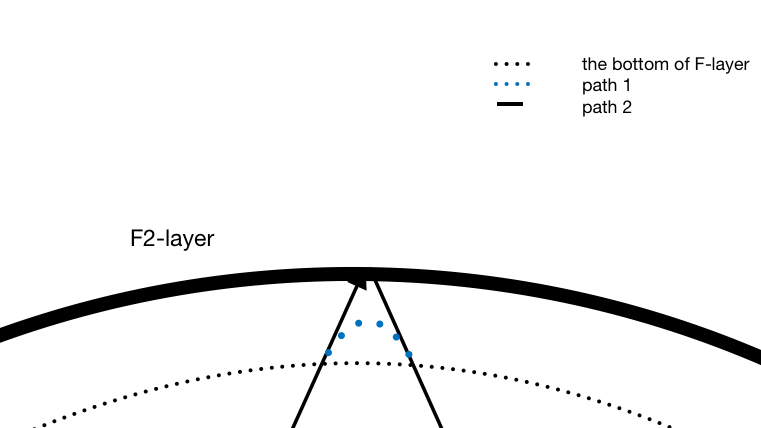
\includegraphics[scale=0.5]{PathinIonosphere}
    \caption{The different path in the ionosphere}
    \label{fig:PathinIonosphere}
    \end{figure}

    And if we consider the general nature of geometrical optics on this Assumption, then we can get such a simplified image(Figure ~\ref{fig:PathinIonosphere}). In the real world, the HF-EM wave's propagating path looks like a parabola (Figure X, \emph{path 1}), however, in our work, we simplyfy this kind of path to the basic form of specular reflection (\emph{path 2}). We took this simplification after making some estimations. First, the EM-wave absorption in the F-layer is first much smaller than absorption in the D-layer, the effect of the F-layer can be neglected in calculating the \textbf{ionospheric absorption} \emph{(which we will discuss in this section's following part)}. Second, if we consider the value of the free-space path loss($L_{fspl}$), the energy lost through \emph{path 1} and \emph{path 2} is negligible because the distance traveled in the ionosphere is much less than the height between the ground and the ionosphere.

    \textbf{Ionospheric absorption loss $L_{a}$} comes from the fact that, when the radio waves passes through, the electrons, ions and neutral molecules in the ionosphere will collide and generate heat in the electromagnetic field. In this process, the electric wave itself loses energy.

    Ionospheric absorption loss is related to the electron number density $N_{e}$, collision rate $v$, the intensity of geomagnetic field and the frequency of radio waves. However, it is difficult to accurately estimate the ionospheric parameters - $N_{e}$, $v$ and so on. Therefore, engineering calculations are often used semi-empirical formula for calculation and prediction\cite{terman1943radio}:

     \begin{equation}\label{eq:IonosphereLoss}
      L_{a} = \frac{677.2}{(f + f_{H})^{1.98} + 10.2}\sum_{i = 1}^{n}\sec\phi_{i} \cdot I_{i}
     \end{equation}
     where:\\
     $\phi$ is the incident angle at the ionosphere;\\
     $I$ is the absorbtion Index;\\
     $N$ refers to the totle number of the hops;\\
     $i$ indicates the current number of hops;

    Like the \emph{path 2} in Figure ~\ref{fig:PathinIonosphere}, the incident angle $\phi$ in the ionosphere can be calculate from the launch angle $\theta$ of the radio waves with some geometrical consideration in Figure ~\ref{fig:Multi_hop_angle}. We can get the result that:

    \begin{figure}[ht]
    \centering
    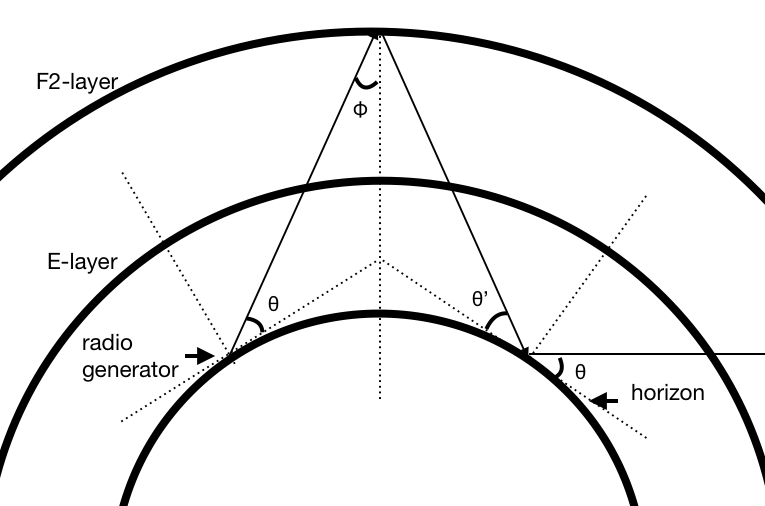
\includegraphics[scale=0.3]{Multi_hop_angle}
    \caption{The geometrical analysis of 'skip' }
    \label{fig:Multi_hop_angle}
    \end{figure}

    \begin{itemize}
      \item From the Figure ~\ref{fig:Multi_hop_angle}, we have $\theta = \theta'$. We will then conclude: the incident angles both at the ionosphere and ground maintain the same at every hops. We will use $\theta$ to represent the luanch angle and $\phi$ as the incident angle at the ionosphere. \\
      \item Considering the Earth's raduis $R_{earth}$ and the height of the F-layer $h_F$, the relationship between two angls is:

        \begin{equation}\label{eq:getPHI}
          \sin\phi = \frac{R_{earth}}{R_{earth} + h_{F}} * \sin(\theta + \frac{\pi}{2})
        \end{equation}

    \end{itemize}



    As for the absorbtion index, we have this result:

     \begin{equation}\label{eq:IonosphereAbsorbtionIndex}
       I = (1 + 0.037 R)(\cos0.881\chi)^{1.3}
     \end{equation}
     Where:\\
     $\chi$ is the electric susceptibility which we have calculated above;\\
     $R$ is the number of \textbf{Sun Spots} which we can get from previous work\cite{dayandyearTECchange};

     The parameters such as $N_{e}$ and $R$ involved in the formula can be obtained by means of ionospheric prediction and mapping. In this paper, we obtained these values of parameters from the NASA's Database.

\subsection{Maximum Usable Frequency}

    In radio transmission maximum usable frequency (MUF) is the highest radio frequency that can be used for transmission between two points via reflection from the ionosphere (skywave or 'skip' propagation) at a specified time, independent of transmitter power\cite{davies1990ionospheric}.

    \begin{equation}\label{MUF_def}
      f_{MUF} = \frac{ 9 \times \sqrt{N_e} }{\cos(\phi)}
    \end{equation}


\section{The Ocean}

  \subsection{Roughness Analysis Method}
    Since we are required to discuss the reflection on a turbulant ocean surface. The turbulent  we need a way to qualify a rough surface like this.

    In mathmatics, a \textbf{fractal} is an abstract object used to describe and simulate natually occuring objects. With this fractal.From the fractal idea, we can express any two-dimensional or high-dimensional image by concrete expressions. In recent years, \textbf{Fractal Geometry} has become a commonly used method to describe a rough surface\cite{lang2015hydraulic,shibuichi1998super}. Based on this method, we can eliminate the randomness of a rough surface and analyze its uniform characteristics.

    We will adapt the multifractal \textbf{detrended fluctuation analysis (MF-DFA)} method from \emph{JW Kantelhardt et al.2002}\cite{kantelhardt2002multifractal}. The detailed steps of this method are not repeated here. Its main idea is that:

    To analyze a rough surface, we usually use the \emph{Fast Fourier Transformation} to sample the surfaces' height. Use the fractal analysis of its parameters: range and variance. Which means we will divide the surface into many sections, and then consider the correlation of the samples in this section we determined. In each section $v$ (from $0$ to $N_s$), with length $s$, we will get an evaluating function $F^2(s,v)$. Using this function in each section, then average over all sections, we will get Equation \ref{eq:F_q} to get the $q$th order fluctuation function:

    \begin{equation}\label{eq:F_q}
      F_q(s) \triangleq {\frac{1}{N_s}\sum_{v=1}^{N_s}[F^2(s,v)]^{q/2}}^{1/q}
    \end{equation}

    The function $F_q(s)$ can be used to describe the surface of a part of the relevance. If we sampling the surface for many times, we can always get a statistical conclusion like this:

    \begin{equation}\label{eq:F_qq}
      F_q(s) \sim s^{H(q) + 1}
    \end{equation}
    Where:\\
    $q$ is a variable real number;\\
    $H$ refers to the Hurst Exponents.

    This conclusion suggests that the $F_q(s)$ itself is obey this distribution which determined by the $q$ and $H$. So these 2 figures are always used to justify the roughness of a surface.

  \subsection{Inverse Roughness Analysis Method}

    If we start from the last step of this MF-DFA method, we may get a rough surface by setting a index $q$, a Hurst Exponent $H$ and a hypothetical waveform function for each little section. So we will get a rough surface following these steps:






  \subsection{Ground Reflection Loss}

\section{Multi-hop HFEW propagation model}



\section{The expansion Applications of the propagation model}

\section{Ships - Consider for Receivers}

\section{Conclusion}
  \subsection{Strengths}
    Huuuuuuge!
  \subsection{Weaknesses}
    Rueeeee
  \subsection{Possible Modifications}
    mmmmmmm


\newpage
% \begin{thebibliography}{99}
%
%     \bibitem{1} D.~E. KNUTH   The \TeX{}book  the American
%     Mathematical Society and Addison-Wesley
%     Publishing Company , 1984-1986.
%     \bibitem{2}Lamport, Leslie,  \LaTeX{}: `` A Document Preparation System '',
%     Addison-Wesley Publishing Company, 1986.
%     \bibitem{3}\url{http://www.latexstudio.net/}
%     \bibitem{4}\url{http://www.chinatex.org/}
%
% \end{thebibliography}

\bibliographystyle{plain}
\bibliography{bib_83451}

\newpage
\begin{appendices}

  \section{First appendix}

    Here are simulation programmes we used in our model as follow.\\

    \textbf{\textcolor[rgb]{0.98,0.00,0.00}{Input Matlab source:}}


\end{appendices}



\end{document}
